%LaTeX Typesetted Notes for MATH1072 (Advanced Multivariate Calculus and
% Ordinary Differential Equations) taught at the University of Queensland,
% Brisbane, 2019 (Semester 2).

% By default, the geometry package should always be on line 7
\documentclass{report}
\usepackage[margin=0.7in]{geometry}

\usepackage{xcolor}
\usepackage{amsmath}
\usepackage{amsthm}
\usepackage{amssymb}
\usepackage{fancyhdr}
\usepackage{lipsum}
\usepackage{graphicx}
\usepackage{wrapfig}

\theoremstyle{definition}
\newtheorem{definition}{Definition}
\newtheorem{example}{Example}

\theoremstyle{plain}
\newtheorem{theorem}{Theorem}
\newtheorem{lemma}{Lemma}
\newtheorem{cor}{Corollary}
\newtheorem{prop}{Proposition}
\newtheorem{conj}{Conjecture}

\theoremstyle{remark}
\newtheorem*{remark}{Remark}
\newtheorem{note}{Note}
\newtheorem{case}{Case}

\pagestyle{fancy}
\fancyhf{}
\rhead{\thechapter}
\lhead{MATH1072 - Advanced Multivariate Calculus and ODEs}
\rfoot{Page \thepage}

\title{Advanced Multivariate Calculus \& Ordinary Differential Equations
(MATH1072) Lecture Notes}
\author{Written by Ismael Khan}
\date{Semester 2, 2019}

\definecolor{term}{RGB}{24, 24, 24}   

\pagecolor{term}
\color{white}

\usepackage{listings}
\usepackage{color}

\definecolor{dkgreen}{rgb}{0,0.6,0}
\definecolor{gray}{rgb}{0.5,0.5,0.5}
\definecolor{mauve}{rgb}{0.58,0,0.82}

\lstset{frame=tb,
  language=Java,
  aboveskip=3mm,
  belowskip=3mm,
  showstringspaces=false,
  columns=flexible,
  basicstyle={\small\ttfamily},
  numbers=none,
  numberstyle=\tiny\color{gray},
  keywordstyle=\color{blue},
  commentstyle=\color{dkgreen},
  stringstyle=\color{mauve},
  breaklines=true,
  breakatwhitespace=true,
  tabsize=3
}

\begin{document}
	\maketitle
	%\tableofcontents
      	\chapter{Ordinary Differential Equations}
	\section{Lecture 1 - Introduction to Dimensional Analysis}
	To descrive real systems quantitatively, we use numbers and units of
	measurement. Eg. 3 meters, 5 years, 10 $ km/h $.
	Each measurable quantity has a certain dimension.
	\subsection{Base dimensions}
	Length $ (L) $, time $ (T) $, mass $ (M) $, other non-mechanical base
	dimensions include temperature; electric charge/current etc.
	\subsection{Derived dimensions}
	Speed $ \displaystyle \frac{L}{T} $, force $ (
	N = M \displaystyle \frac{L}{T^2}) $, energy $ (J = M \displaystyle
	\frac{L^2}{T^2}) $. The dimensions of the terms added on both sides
	must be equal. This is known as the equation being
	\textit{dimensionally homogenous}. We can use the dimensional
	homogeneity to make dimensional estimates for certain quantities
	(order of magnitude, not exact prediction)
	\section{Lecture 2 - Dimensional Analysis}
	\section{Lecture 3 - Introduction to Differential Equations}
	\noindent Generally, an ordinary differential equation (ODE) is represented as:
	$$ F(t,y(t), y'(t), y''(t), ...)  = 0 $$
	For Instance, Newton's Law
	$$ m \frac{d^2 r}{dt^2} = F $$
	Induction Law:
	$$ RI + L \frac{dI}{dt} + \frac{1}{c} $$
	Population:
	$$ \frac{dP}{dt} = rP(1- \frac{P}{k})$$
	Maxwell's Equations:
	\begin{align*}
		\nabla \cdot \bar{E} &= \frac{1}{\rho} \varepsilon_0 \\
		\nabla \cdot \bar{B} &= 0 \\
		\nabla \times \bar{E} &= \frac{\delta B}{\delta t} \\
		\nabla \times \bar{B} &= \mu_0 J + \mu_0 \varepsilon_0 \frac{\delta E}{\delta t}
	\end{align*}

	Navier-Stokes: (Modelling velocity of fluids in space)
	$$ \frac{\delta \bar{v}}{\delta t} = \overline{v} \nabla \overline{v} = ? $$

	Schrodinger Wave Equation:
	$$ i\hbar \frac{\delta \psi}{\delta t} = \Big[ \frac{-\hbar}{2m} \nabla^2 + V(r)\Big]\psi$$
	$$ \psi = ? $$
	We generally have:
	$$ F(t, y(t), y'(t), ...) = 0,\; y(t) = ? $$
	Where the order of ODE $ = $ order of the highest derivative. Take the
	equation $y' = y$, the solutions are $ y = e^t $, $ y = 0 $ and
	$ y = ce^t $. However the latter expression encapsulates the former, so
	$ y(t) = ce^t $ is known as the general solution where $ c \in
	\mathbb{R} $. The general solution is not unique. \\\\
	If you take an ODE and add some initial condition, then the solution is a unique result. For Instance take the ODE $ y' = y $ and say that $ y(0) = 1 $, then we achieve a unique solution of $ c = 1 $, $ y = e^t $.
      \section{Lecture 4 - Ordinary Differential Equations}
      \subsection{Equilibrium Solutions}
      An equilibrium solution (steady state solution) of an ODE (if such
      solution exists) is a constant solution $ y(t) = c $ which satisfies the
      ODE (for any $ t $). 
      \begin{example}
	Take $ y' = f(t,y) $, the equilibrium solution 
	$$ f(t,y = c) = 0 $$
      \end{example}
      \noindent This implies that the slope at $ y = c $ must be 0 for
      a function defined on a $ (t,y) $ plane

      \begin{example}
      $ y' = y $, $ y = 0 $ is an equilibrium solution.
      \end{example}

      \begin{example}
	$ y' = y(1-y) $m $ y = 0 $ and $ y = 1 $ are equilibrium solutions
      \end{example}
      \noindent Slope fields can visualised with Mathematica using StreamPlot
      (or VectorPlot). The vector flow of a field corresponding to $ f(t,y)
      $ is $ \{1, f(t,y)\} $ since the flow in the horizontal direction $ (t)
      $ has a constant rate (the flow of time) which can be set to $ 1 $, the
      vertical flow is $ f(t,y) $.

      \subsection{Stability of equilibrium solutions}
      If the solutions starting in condition a small neighbourhood of an
      equilibrium solution $ (y = c) $ converge towards the equilibrium solution
      for large $ t $, then the equilibrium solution $ y = c $ is stable.

      \begin{example}
	$ y' = y $, the equilibrium solution $ y = 0 $ is unstable (for $ y'
	= -y $, $ y = 0 $ is stable)
      \end{example}

      \begin{example}
	$ y' = y(1-y) $, $ y = 0 $ is unstable, but $ y = 1 $ is stable.
      \end{example}

%Indenting LaTeX files? Is it a mandatory thing? Spacing can cause actual
      %typsetting errors but Indenting does not...
      % Regardless, Vim decides to indent for me anyways because of the
      % document environment.
      %

\section{Lecture 5 - Stability of ODE's}
\subsection{Condition for stability of equilibrium soltuions}
Using a Taylor Series approximation of $ f(t,y) $ near the equilibrium solution
$ y = c $, assume $ f(t,y) = f(y) $ for simplicity
$$ f(y) \approx f(c) + f'(c)(y-c) + \frac{1}{2} f''(c)(y-c)^2 + ... $$
Where $ y = c  $ is the equilibrium solution $ f(c) = 0 $, thus
$$ y'(t) = 0 + f'(c)(y-c) + \frac{1}{2} f''(c)(y-c) + ... $$
Take $ u = y -c $, then $$ u' = f'(c)u + ... $$
Implying
$$ u(t) = Ae^{f'(c) t} $$
If $ f'(c) > 0 $, $ y = c $ is unstable. If $ f'(c) < 0 $, $ u(t) \to 0 $,
$ y(t) \to c $ thus $ y =c  $ is stable.
\subsection{Euler's Method}
An iterative operation which models $ y_k \approx y(k\cdot \Delta t)$. Given
$ y' = f(t,y) $, $ y(0) = c$ 
\begin{align}
  y'(t) &\equiv \lim_{\Delta \to 0} \frac{y(t+\Delta) - y(t)}{\Delta}\\ &\approx \frac{y(t+\Delta) - y(t)}{\Delta}
\end{align}
As it is an iterative method, $ y_{k+1} = y_{k} + f(t_k, y_k) $
$$ \frac{y(t_{k+1})-y(t_k)}{\Delta} \approx f(t_k, y_k) $$
\begin{example}
  Given $ y' = 2t $, $ y(t) = ? $, $ y(0) = 0 $. By Euler's Method
  \begin{align}
    N &= 1, \; \Delta = 1 \\
    N &= 2, \; \Delta = \frac{1}{2}\\
    N &= 4, \; \Delta = \frac{1}{4}\\
    N &= 10 \; \Delta = \frac{1}{10}
  \end{align}
\end{example}

\section{Lecture 6 - Continuation of Euler's Method}
\subsection{Error Generated in Euler's Method}
Assume $ y(t_k) = y_k $, the error is represented with the taylor series
approximation 
\begin{align*}
  \Big | y_{k+1} - y(t_k + \Delta) \Big | &= y(t_{k+1}) = y(t_k)
+ y'(t_k)\Delta + \frac{1}{2}y''(t_k) \Delta^2 + ... \\
  y_{k+1} &= y_k + f(t_k, y_k)\Delta
\end{align*}
Thus $$ \text{error} = |y_{k+1} - y(t_k + \Delta)| \propto \Delta^2 $$
However generalized for $ N $ steps,
\begin{align*}
  N\cdot|y_{k+1} - y(t_k + \Delta)| &\propto \Delta^2 \cdot N \\
				    &\propto \Delta^2 \cdot \frac{1}{\Delta}
				    \propto \Delta
\end{align*}

$$ y_{k+1} = y_k + \frac{1}{2}\Big[f(t_k, y_k) + f(t_{k+1}, y_{k+1}) \Big]
\Delta$$

\section{Lecture 7 - Solving Linear First Order ODEs}
\[y' = f(t,y), y(0) = y_0\]
\[t \in [0,t_{max}]\]

\begin{enumerate}
      \item Euler's Method
      \[y_{k+1} = y_k + f(t_k, y_k) \Delta\]
      Where total error \( \propto \Delta\)
      \item Heun Method (Revised Euler's Method)
      \[\begin{cases}
            y_{k+1} = y_k + f(t_k, y_k) \Delta \\
            y_{k+1} = y_k + \frac{1}{2} [f(t_k, y_k) + f(t_k + \Delta, y_{k+1})]
      \end{cases}\]
      Where total error \(\propto \Delta^2\). Note that Heun Method will possibly show in
      Assignment 3.
\end{enumerate}
\subsection{Runge Kutta Method}
\begin{align*}
      p_1 &= f(t_k, y_k) \Delta\\
      p_2 &= f(t_k + \frac{\Delta}{2}, y_k + \frac{p_1}{2})\Delta\\
      p_3 &= f(t_k + \frac{\Delta}{2}, y_k + \frac{p_2}{2})\Delta\\
      p_4 &= f(t_k + \frac{\Delta}{2}, y_k + p_3) \Delta
\end{align*}
for \[y_{k+1} = y_k + \frac{1}{6} p_1 + \frac{1}{3} p_2 + \frac{1}{3} p_3 + \frac{1}{6}p_4 + ...\]
\subsection{Adaptive Step Size}
Fixed step size is mostly inefficient in most cases, so we use an adaptive step size
for numerical methods to achieve better approximations.

\subsection{Coupled Systems}
\begin{align*}
      y' &= f(t,y_1, y_2) \\
      x' &= g(t, y_1, y_2) 
\end{align*}
\[x(t) = ? \; y(t) = ?\]
In the context of Euler's Method
\[\begin{cases}
      x_{k+1} = x_k + f(t_k , x_k, y_k)\Delta\\
      y_{k+1} = y_k + g(t_k, x_k, y_k)\Delta
\end{cases}\]

\subsection{Analytical ODE Solutions}
\subsubsection{Linear First Order ODE's}
By definition,
\[y(t) = f(t)y(t) + g(t)\]
is generally the standard form of a linear first order ODE. Note that 
\[y'(t) = f(t)y(t)\]
is a special case of a linear first order ODE that is separable.

\begin{example}
      \[ty' + y = t\cos t\]
      Observe that, by the product rule for differentiation, \(ty' + y = (ty)'\).
      \begin{align*}
            (ty)' &= t\cos t\\
            \int (ty)' dy &= \int t \cos t dt\\ 
            ty &= t\sin t - \int \sin t dt \\
            ty &= t\sin t + \cos t + c\\
            \therefore y &= \frac{t\sin t + \cos t}{t} + \frac{c}{t}
      \end{align*}

      
\end{example}
% Lectures 9-11 need to be updated to the notes. Refer to blackboard content
% and 

\section{Lecture 8 - Applications of First Order ODEs}
Common applications of first order ODEs are
\subsection{Radioactive Decay}
The particles of a radioactive material decay spontaneously in a stochastic
process. The total mass of the radioactive atoms decrease with time. We can represent this as 
$$ \frac{dM}{dt} = -kM $$
For $ M(t) $ to represent the mass of the radioactive material over time $ t $.
% This is all one line of text, maybe add some line breaks...
\noindent
Clearly the solution to this is 
$$ M(t) = M_0 e^{-kt} $$
Note that there is a limitation to this ODE Model. We assume that the mass changes \underline{continuously} in time. Whereas in reality it 
changes in discrete steps following individual decay events. However 
for the macroscopic mass, the number of particles is much larger, so we can neglect the discrete jumps and assume a continuous deterministic model. Which works well for most cases.
\\ \par
The lifetime of particles varies, however we can categorize them
with their average lifetime. We do this by asking how long it
takes for a particle to reduce to half of the initial value.
To obtain a more accurate value for average lifetime, consider
grouping the lifetime of particles into discrete "bins". If the
number of particles with lifetime in $ [t_j, t_j + \Delta] $
is $ N_j $, then the average lifetimes is represented as
$$ \sum N_j = N_0 $$
$$ \tau \approx \frac{ \displaystyle \sum t_j N_j}{\displaystyle \sum N_j} $$
If the number of particles decreases exponentially
$$ N(t) = N_0 e^{-kt} $$
Then the number of particles lost in an interval $ [t_j, t_j + \Delta] $ is 
$$ N_j = N[t_j] - N[t_j + \Delta] $$
Or
$$ N_j = \frac{N(t_j) - N(t_j + \Delta)}{\Delta} \cdot \Delta
\approx - N'(t)\Delta$$
Taking $ \Delta \to 0 $. The sum for calculating the average lifetime turns into an integral.
$$ \tau = \frac{1}{N_0} \int_0^\infty  t(-N'(t)) \; dt = 
\int_0^\infty te^{-kt} \; dt = \frac{1}{k}$$
\subsection{Protein Synthesis and Degradation}
Seriously who cares. I probably should write these notes though
\section{Lecture 9 - Continuation of Protein Synthesis and Degradation}
The concentration of a protein $ C(t) $ that is synthesised at a constant rate
$ S $, $ k $ for the degradation rate.
$$ \frac{dC}{dt} = S - kC $$
We can see that the equilibrium state is at $ C = \frac{S}{k} $, the ODE is
seperable, so the general solution is as follows
$$ \int \frac{dC}{S-kC} \; = \int dt $$
And then... Poof! By the magic of Applied Mathematics, we achieve the general
solution
$$ C(t) = \frac{S}{k} + ce^{-kt} $$
Assume the initial value such that for $ C(t=0) = C_0 $, then the general
solution
$$ C(t) = \frac{S}{k} + \Big (C_0 - \frac{S}{k} \Big) e^{-kt} $$

% Insert graphic from Lecture Notes???

\section{Lecture 10 - Heat Transfer}
The heat flow (energy transferred per unit time) between two object of
different temperature is proportional to the temperature difference between the
two object (the heat flows from the higher to the low temperatures until it
equilibrates). Thus the rate of change of the body temperature is proportional
to the temperature difference between the body and the environment $ T_{env}
$ (air). 
$$ \frac{dT}{dt} = - k(T-T_{env})  $$
$$ T(t) = T_{env} + (T_0 - T_{env})e^{-kt} $$
Setting $ t = 0 $ solves for $ T_0 $ and $ T_{env} $ should be predefined. The
parameter $ k $ is a proportionality constant and is difficult to represent
with a model (at this level)
\subsection{Electric circuit with resistance and inductance}
$ R $ resistance, $ L $ inductance in series, $ E(t) $ external voltage source
$ = $ the sum of the voltage drops over the resistance + the inductance.
The ODE for the current $ I(t) $,
$$ E(t) = RI + L \frac{dI}{dt} $$
\subsection{Population Dynamics}
The rate of change of the population $ P(t) $ is proportional with the actual
current population 
$$ \frac{dP}{dt} = kP $$, $$ P(t) = P_0 e^{kt} $$
The $ k $ parameter in this model is the cell division rate constant. Ideally,
bacteria can divide every 20 minutes.
\section{Lecture 11 - Continuation of Population Dynamics}
To balance out the growth of population due to reproduction we can also include
a loss term due to death. The number of individuals dying per unit time is also
proportional to population size $ P $
$$ \frac{dP}{dt} = kp - dP = (k-d)P = \rho P$$
$$ P(t) = P_0 e^{\rho t} $$
This modified population model still doesn't have a stable equilibrium state.
The solution grows or decays exponentially depending on the sign of $ \rho
= k - d $ which is the \textbf{net reproduction rate constant}.
It is expected that a population should stabilise after some time in a stable
equilibrium; where repoduction and death balance out.
\par The thing missing from this model is that we assumed $ k $ and $ d $ are
constant parameters, but the birth and death rates may be dependant on several
external factors (e.g. food, habitat) and this may be dependent on the size of
the population $ r $, $ k $ (or $ \rho $) are functions of $ P $. 
\\\\
Thus a modified nonlinear population model
$$ \frac{dP}{dt} = \rho (P) P $$
Where the exact form of the function $ \rho (P) $ depends on the problem in
question that we want to model. In general $ \rho (P) $ is a decreasing
function (less resources available when the population increases, which slows
down reproduction and/or increases death rate).
\\\\
The simplest functional form for a decreasing $ \rho (P) $ is a linear function
$$ \frac{dP}{dt} = \rho \Big (1 - \frac{P}{K} \Big ) P $$
This is known as the \textbf{Logistic Equation}, where $ \rho  $ is a constant
(maximum net reproduction rate), $ K $ is the carrying capacity (the maximum
sustainable population size). The net reproduction changes sign from positive
to negative when $ P = K $. The equilibrium solutions of this model are 
\begin{itemize}
  \item $ P^* = 0 $; unstable
  \item $ P^* = K $; the derivative of RHS at $ P = K $ is $ < 0 $ implying
    stable equilibrium state.
\end{itemize}
The exact solution to this ODE (seperable ODE) with initial condition $ P(0)
= P_0 $ is 
$$ P(t) = K \frac{1}{1+\Big( \frac{K}{P_0} - 1\Big) e^{-\rho t}} $$
For a long time $ t \to \infty $, the solution $ P(t) $ converges to the stable
equilibrium. Assume that $ P $ describes a fish population and there is an
additional loss rate due to fishing.
$$ \frac{dP}{dt} = \rho \Big (1 - \frac{P}{K}\Big ) P - f $$
$ f $ is a constant parameter; the amount of fish harvested per unit time.
\subsubsection*{Question:}
How does the fishing rate $ f $ modify the state equilibrium of the population?
How should the function $ P^* (f) $ look graphed?. Is there any qualitative
(dramatic) change of the equilibrium as $ f $ is modified or only a smooth
transition; are there any bifuractions?
\section{Lecture 12 - ODE Models of Population Dynamics}
\subsection{Bifuraction}
Consider the Differential equation $ \displaystyle \frac{dy}{dt} = f(y;p)
$ where $ p $ represents constant parameters. The equilibrium solutions are the
roots of the equations $ f(y) = 0 \implies \displaystyle \frac{dy}{dt} $ which
will depend on the parameters. Bifuraction diagrams are qualitative changes of
the solutions happening when a parameter $ p $ is varied, i.e the change in the
number of stability type of the equilibria. A \textbf{bifuraction diagram}
plots and shows the solutions of branches $ y^*(p) $. 
\subsection{Logistic populations dynamics}
Consider the equation 
$$ \frac{dP}{dt} = \rho \Big (1 - \frac{P}{K} \Big ) P $$
Introduce non-dimensional variables for $ P $ and $ t $ in order to reduce the
number of parameters in the problem. Choose $ P' = \frac{P}{K}  $ and $ t'
= \rho t $. 
$$ \frac{dP'}{dt'} = (1-P')P' $$
The non-dimensional problem does not have any parameters. This shows that we
can't have any bifuractiosn when we modify $ K $, and $ \rho $ as those are all
mathematically equibva;lent problems they can only differ by strecthing or
compeessing the axis $ P $ and $ t $. Now consider the equation 
$$ \frac{dP}{dt} = \rho \Big (1 - \frac{P}{K} \Big) P - F $$
Introduce the same non-dimensional variables for $ P $ and $ t $;
($ P' = \frac{P}{K} $ and $ t' = \rho t $).
$$ \frac{dP'}{dt'} = (1-P')P' - \frac{F}{\rho K} $$
Denoting $ \displaystyle \frac{F}{\rho K} = F' $, $ F' $ cannot be elimated by
using non-dimensional variable, so the problem has 1 real parameter $ \implies
$ it may have qualitatively different solutions when $ F' $ is varied.
\subsection{Harvesting at a constant rate}
$$ \frac{dP'}{dt'} = (1-P')P' - F' $$
How does the equilibria change when $ F' $ is varied? ($P'^*(F') = ? $ ). Solve
it graphically by following the intersections of the two terms on the RHS as
$ F' $ is varied?

\section{Lecture 13 - Systems of Coupled 1st Order ODEs}
$$ y'_1 = f(y_1,y_2), \; y'_2 = g(y_1, y_2) $$
$ y_1(t) = ? $ and $ y_2(t) = ? $. There is no general method for finding
solutions analytically for coupled systems of ODEs (except linear systems), but
often the important information is related to the equilibrium states of the
system. The equilbrium solutions $ (y_1^*, y_2^*) $ are the solutions of the
algebraic system of simultaneous equations:
$$ f(y_1, y_2) = 0 , \; g(y_1, y_2)  = 0 $$
\subsection{Dynamics of interacting populations}
\begin{example}
  Prey $ (P) $ and predator $ (R) $ population dynamics.
  $$ \frac{dP}{dt} = \rho P \Big (1 - \frac{P}{K}\Big) - aPR $$
  $$ \frac{dR}{dt} = bPR - dR $$
  Given $ \displaystyle \rho P\Big ( 1 - \frac{P}{K}\Big ) $ is the prey without predator,
  $ aPR $ is the prey-predator interaction and $ bPR - dR $ is the death of
  predator.
\end{example}
Non-dimensionalize the sytem by introducing new dimensionaless variables $ P'
= \displaystyle \frac{P}{K} $, $ t' = \rho t $ (done similarly for the logistic equation) and
choose $ R' = \displaystyle \frac{a}{\rho} R$. 
$$ \frac{dP'}{dt'} = P'(1-P') - P'R' $$
$$ \frac{dR'}{dt'} = \frac{bK}{\rho} P'R' - \frac{d}{\rho} R' $$
$$ \frac{dR'}{dt'} = \alpha P' R' - \beta R' $$
The non-dimensionalization shows that the behaviour of the solution can only
depend on the two new parameters $ \alpha = b \displaystyle \frac{K}{\rho}
$ and $ \beta = \displaystyle \frac{d}{\rho} $
\section{Lecture 14 - Second Order Differential Equations}
$$ f(y'', y', y,t) = 0, \; y(t) = ?$$
\begin{example}
  Newton's Law $ F = ma $, where $ a $ is the acceleration. (second derivative
  of coordinate function $ a = x''(t)) $
\end{example}
Many partial differentials contain second derivates over spatial coordinates.
There is no general way to solve nonlinear second order ODEs analytically,
however we can solve them numerically.
\par 
To solve numerically, we can rewrite it into the form of two coupled first
order ODEs by introducing an unknown function defined as $ y' = v $. Then $ v'
= F(v,y,t)$ and $ y' = v $ forms a coupled system, needs to be complemented
with initial conditions $ y(t=0)$ and $ v(t=0) = y'(t=0) $
\subsection{Solving linear 2nd order ODEs analytically}
Some types of linear 2nd order ODEs may be solved analytically. A general form
of a analytically solveable 2nd order ODE may be
$$ y'' + p(t) y' + q(t) y = r(x) $$
Can be classified as homogenous if $ r(x) = 0 \; \forall x $. Constant
coefficients if $ p(t)  $ and $ q(t) $ are constants. For homogenous ODEs
($ r(x) = 0 $), we can use the \textbf{Principle of superposition} for
construction the general solution.
\\\\
If $ y_1(t) $ and $ y_2(t) $ are two linearly independent solutions of the
homogenous linear 2nd order ODE then any linear combination $ y(t) = c_1 $.
What?
\subsection{Method of Reduction of Order}
Assume that we have a solution $ y_1(t) $ that satisfies a linear homogenous
ODE $ \implies $ then the reduction of order method leads to a problem of
a lower order ODE for finding the other/general solution. The steps for solving
with reduction of order method is as follows
\begin{enumerate}
  \item $ y'' + p(t) y' + q(t) y = 0 $
  \item Assume that $ y_1 (t) $ is a solution.
  \item Look for solutions of the form $ y = u(t)y_1(t) $
  \item Substitute into the equation.
  \item $ (u y_1)'' + p(t) (u y_1)' + q(t) u y_1 = 0 $
\end{enumerate}
\section{Lecture 15 - Solving 2nd Order ODES}
Suppose we have a linear $ 2^{nd} $ order ODE $ f(y'', y', y, t) = 0 $. Suppose
we are solving for the general solution $ y(t) $. If $ f $ is homogenous and
constant-coefficient, the ODE is of the form $ y'' + ay' + by = 0  $. As
a function that remains the same (same for a multiplicative constant) is $ e^t
$, we can guess $ y(t) = e^{\lambda t} $ is a solution for some $ \lambda $.
\begin{align*}
  y'' + ay' + b &= (e^{\lambda t})'' + a(e^{\lambda t})' + be^{\lambda t}\\
  0 &= \lambda^2 e^\lambda t + \lambda a e^{\lambda t} + be^{\lambda t}\\
  0 &= e^{\lambda t} (\lambda^2 + a\lambda + b)
  \intertext{Note that $ \lambda^2 + a\lambda + b = 0 $ is the characteristic
  equation of an ODE}
\end{align*}
$$ \implies \lambda_{1,2} = \frac{-a \pm \sqrt{a^2 - 4b}}{2} $$
Thus $ e^{\lambda_1 t} $ and $ e^{\lambda_2 t}$ are linearly independent
solutions and the general solution is $ y(t) = c_1 e^{\lambda_1 t} + c_2
e^{\lambda_2 t} $ for some $ c_1, \; c_2 $. However, this is only the case if
$ \lambda_1 \neq \text{something} $ ($ 4b < a^2 $). 
\\\\
If $ 4b = a^2 $, then $ \lambda_1 = \lambda_2 = \lambda $ and we obtain only
one solution $ \lambda^{\lambda t} $. With this, we can use reduction of order.
As $ y_1(t) = e^{\lambda t} $ is a solution, let $ y(t) = u(t) e^{\lambda t} $.
Thus $ y'' + ay' + by = 0 $
$$ \implies (ue^{\lambda t})'' + a(ue^{\lambda t})' + bue^{\lambda t} = 0 $$
\begin{align*}
  (u'e^{\lambda t} + \lambda u e^{\lambda t})' + a(u'e^{\lambda t} + \lambda
  u e^{\lambda t}) + bue^{\lambda t} &= 0\\
  u''e^{\lambda t} + \lambda u' e^{\lambda t} + \lambda u' e^{\lambda t}
  + \lambda^2ue^{\lambda t} + au' e^{\lambda t} + a\lambda u e^{\lambda t}
  + bue^{\lambda t} &= 0\\
  u'' + 2\lambda u' + \lambda^2u + au' + a\lambda u + bu &= 0
\end{align*}
However note that $ \lambda = \displaystyle \frac{-a}{2} $, $ 4b = a^2 \implies
b = \displaystyle \frac{a^2}{4}$
$$ u'' - au' + \frac{a^2}{4}+ au' - \frac{a^2}{2}u + \frac{a^2}{4}u = 0$$
\begin{align*}
  &\implies u'' = 0\\
  &\implies u(t) = c_1t + c_2
\end{align*}
for some $ c_1 $, $ c_2 $. Thus the general solution is
$$ y(t) = u(t) e^{\lambda t} = (c_1 t + c_2) e^{\lambda t} $$
If we obtain no solutions $ (4b > a^2) $ in the real set, we get two complex
conjugate roots.
$$ \lambda_{1,2} = \frac{-a}{2} \pm \frac{\sqrt{4b - a^2}}{2}i = \alpha \pm
\beta i $$
We get the general solution
\begin{align*}
  y(t) &= c_1 e^{(\alpha + \beta i)t} + c_2 e^{(\alpha - \beta i)} \\
       &= c_1 e^{\alpha t} e^{\beta i t} + c_2 e^{\alpha t} e^{-\beta i t}
\end{align*}
However, $ e^{i\beta t} = \cos (\beta t) + i \sin (\beta t) \implies y(t)
= e^{\alpha t} (c_1 \cos(\beta t) + c_1 i \sin (\beta t) + c_2 \cos(-\beta t)
+ i \sin (-\beta t) $
\begin{align*}
  y(t) &= (c_1 + c_2 e^{\alpha t} \cos(\beta t) + (c_1 - c_2) ie^{\alpha t}
  \sin (\beta t)\\
  \intertext{Let $ A = c_1 + c_2 $ and $ B = (c_1 - c_2)i $ }
  y(t) &= Ae^{\alpha t} \cos (\beta t) + B e^{\alpha t} \sin (\beta t)\\
       &= e^{\alpha t} (A\cos (\beta t) + B \sin (\beta t))
\end{align*}
\section{Lecture 16 - Constant-coefficient Non-Homogenous}
Suppose we have an ODE $ y'' + p(t)y' + q(t)y = r(t) $ and we are attempting to
solve for $ y(t) $. This is a constant coefficient non homogenous linear order
$ 2^{nd} $ oder ODE. (if $ p(t) $, $ q(t) $ are constant). Let $ L(x) = x''
+ px' + qx $. Suppose we have two linearly independent solutions $ y_1(t),
y_2(t) $. Thus $ L(y_1) = L(y_2) = r \implies L(y_1) - L(y_2) = 0 $. As the ODE
is linear $ \implies $ $ L $ is linear, $ L(y_1) - L(y_2) = L(y_1 - y_2) = 0 $.
This is a homogenous ODE and can be easily solved
\paragraph{Steps:}
\begin{enumerate}
  \item Solve the corresponding homogenous ODE $ (r=0) \to y_n = c_1 y_n + c_2
    y_k $
  \item Find solution $ y_p $ (reduction of order) $ \to y_p = u(t)y_{k_1} $
  \item General case is $ y(t) = y_p + y_n $
\end{enumerate}
\begin{example}
  Solve for $ y(t) $ given $ y'' + y' - 2y = t^2 - 2t + 3 $
  \begin{enumerate}
    \item Solve $ y'' + y' - 2y = 0 $, characteristic equation is $ \lambda ^2
      + \lambda - 2 = 0$. Implying
      $$ (\lambda+2) (\lambda - 2) = 0 $$
      Thus $ \lambda_1 = -2 $ and $ \lambda _2 = 1 $, therefore
      $$ y_n (t) = c_1 e^{-2t} + c_2 e^t $$
    \item Reduction of Order: as $ y_1(t) = e^t $ is a solution we have
      a linearly independent solution $ y_p(t) = u(t)e^t $. Subbing in 
      \begin{align*}
	(ue^t)'' + (ue^t)' - 2ue^t &= t^2 - 2t + 3\\
	u''e^t + 2u'e^t t + ut^2 e^t + u' e^t + ute^t - 2ue^t &= t^2 - 2t
	+ 3 \\
	u'' + 2u't + ut^2 + u' + u5 - 2u &= (t^2 - 2t + 3)e^{-t}
      \end{align*}
      $$ \implies y(t) = c_1 e^{-2t} + c_2 e^t - \frac{t^2}{2} + \frac{t}{2}
      - \frac{7}{4} $$
  \end{enumerate}
\end{example}

\section{Lecture 17 - }

\section{Lecture 18 - Applications of 2nd order ODEs}
\subsection{Mechanical/Electrical Ossiclators}
\textbf{SMALL ANGLE TIME}
$$ \sin (\theta) = \theta $$
$$ m \frac{dy}{dt} = -mg + kdy  $$
\begin{example}
  Given a pendulum,
  $$ m \frac{d^2y}{dt^2} = - ky $$
  $$ y(0) = y_0, \; y'(0) = 0 $$
\end{example}
\begin{align*}
  my'' + ky &= 0\\
  y'' + \frac{k}{m}y &= 0\\
  \intertext{Denote $ a = \displaystyle \frac{k}{m} $}
  y'' + ay &= 0 \implies \lambda^2 + a = 0 \\
  \therefore y &= e^{\lambda t} 
  \intertext{For $ \lambda = \pm i \sqrt{a} $}
  y(t) &= A \cos (\sqrt{a} t) + B \sin (\sqrt{a} t)
\end{align*}
However with this model there is no dampining over time. 
$$ m \frac{d^2y }{dt^2} = -ky - \gamma y' $$
\begin{align*}
  y'' + \Big ( \frac{\gamma}{m}\Big) y' + \Big ( \frac{k}{m} \Big) y &= 0\\
  \intertext{Denoting $ \displaystyle \frac{\gamma}{m} = b $ and
  $ \displaystyle \frac{m}{k} = a $}
  y'' + by' + ay &= 0
  \intertext{If $ b^2 > 4a $, $ \lambda_1, \lambda_2 < 0 $, if $ b^2 < 4a $,
  $ \lambda_{1,2} = \displaystyle \frac{-b}{2} \pm i\sqrt{4a-b^2} $}
\end{align*}
\chapter{Multivariable Calculus}
\textbf{Foreword:} From around this point onwards I began to lost track on the
exact Lectures that these notes come from, so they are going to be referred by
weeks.
\section*{Week 7}
\section{Introduction to Multivariate Calculus}
\subsection{Review of one-variable case}
Let $ f: D \to \mathbb{R} $ be a function with a domain $ D $ an open subset of
$ \mathbb{R} $. For $ a \in D $ we say that the limit $ \displaystyle \lim_{x
\to a}  f(x) $ exists if and only if 
\begin{enumerate}
  \item The limit from the left exists
  \item the limit from the right exists
  \item these two limits coincide etc.
\end{enumerate}
    $$ \lim_{x \to a^-} f(x) = \lim_{x \to a^+}  f(x) $$
    Furthermore if the limit exists and is equal to the actual value of
    $ f $ at $ a $.
    $$ \lim_{x\to a^-}  f(x) = \lim_{x \to a^+}  f(x) = f(a) $$
    We say that $ f $ is continuous at $ x = a $. If $ f $ is continuous on all
    $ D $, we say that $ f $ is continuous function on $ D $
    \subsection{The two-variable case}
    When $ f $ is a function of more than one variable, the situation is more
    subtle. There are more than two ways to approach a given point of interest.
    \begin{example}
    Consider the function
    $$ f(x,y) = \frac{x^2}{x^2 + y^2} $$
    with domain given by $ \mathbb{R}^2 \setminus {(0,0)} $
    \end{example}
    Approaching the origin along $ y = 0 $, if $ x \neq 0  f(x,0)
    = \displaystyle \frac{x^2}{x^2 + 0} = 1$. Then 
    $$ \lim_{x\to 0} \; f(x,0) = 1 $$
    If $ y \neq 0  $, $ f(0,y) = \displaystyle \frac{0}{0+y^2} = 0 $. Then,
    $$ \lim_{y \to 0}  f(0,y) = 0 $$
    Thus $ \displaystyle \lim_{(x,y) \to (0,0)} f(x,y) $ does not exist, as
    $ \displaystyle \lim_{x\to 0} f(x,0) \neq \displaystyle \lim_{y\to 0}
    f(0,y) $. In general, for the limit $ \displaystyle \lim_{(x,y) \to (a,b)} 
    f(x,y)$ to exist, it is neccessary that every parth in $ D $ approaching
    $ (a,b) $ gives the same limiting value ($ (a,b) $ may not neccesarily be
    inbluetooth usbc $ D $). This gives a method for finding if a limit does not exist for
    multivariate limits.
    \[
      \text{If } \displaystyle \begin{cases}
      f(x,y) \to L_1 \text{ as } (x,y) \to (a,b) \text{ along the path } C_1
      \in D\\
      f(x,y) \to L_2 \text{ as } (x,y) \to (a,b) \text { along the path } C_2
      \in  D
    \end{cases} 
  \]
    \begin{remark}
  The above notation is somewhat deficient and perhaps one should write
  $$ \lim_{(x,y) \to (a,b)} f(x,y) $$
  to indicate that only paths $ D $ terminating in $ (a,b) $ (which itself may
  or may not be in $ D $) are considered. For instance,
  $ f(x,y) = x^2 + y^2 $ with $ D = \{(x,y): x^2 + y^2 < 1\} $, then
  $ \displaystyle \lim_{(x,y) \to (1,0)}  f(x,y) $ exists and is 1. However if 
 \[ 
    \begin{cases}
      x^2 + y^2 &\text{ for } D = \{(x,y): x^2 + y^2 < 1\}\\
      0 &\text{ for } D = \{(x,y): x^2 + y^2 > 1\}
    \end{cases}
    \]
    then $ \displaystyle \lim_{(x,y) \to (1,0)} f(x,y) $ does not exist.
  \end{remark}

    \section{Lecture 20 - Continuation of Functions of Multiple Variables}
    Generally, we write $ \displaystyle \lim_{(x,y) \to (a,b)}  f(x,y) = L $ to
    mean the values of $ f(x,y) $ approach $ L $ as the point $ (x,y)
    $ approaches $ (a,b) $ along any path in the domain $ f $. That is, we can
    make the value of $ f(x,y) $ as close to $ L $ as we like by taking $ (x,y)
    $ sufficiently close to $ (a,b) $. This is formalised through the following
    definition
    \begin{definition}
    Let $ f $ be a function of two variables whose domain $ D $ includes points
    arbitrarily close to $ (a,b) $. 
    \\\\
    Then we say that the limit of $ f(x,y) $ as $ (x,y) $ approaches $ (a,b)
    $ is $ L $ and we write
    $$ \lim_{(x,y) \to (a,b)} f(x,y) = L $$
    if for every number $ \varepsilon > 0 $, $ \exists \delta > 0 $ such that
    if $ (x,y) \in D $ and $ 0 < \sqrt{(x-a)^2 + (y-b)^2} < \delta $, then
    $ |f(x,y) - L| < \varepsilon $. Where $ |f(x,y)-L| $ can be described as
    the distance between $ f(x,y) $ and $ L $ in $ \mathbb{R} $. The
    $ \sqrt{(x-a)^2 + (y-b)^2} $ is the distance between $ (x,y) $ and $ (a,b)
    $ in $ \mathbb{R}^2 $. The definition is essentially saying that the
    distance between $ f(x,y)  $ and $ L $ can be made arbitrarily small by
    making the distance between $ (x,y)  $ and $ (a,b) $ sufficiently small,
    \textbf{but not 0}.
    \end{definition}

    \section{Lecture 23 - Partial Derivatives}
    Consider the surface $ z = f(x,y) = 1-x^2 - y^2 $ and the point
    $ P = (1,-1,-1) $ on the surface. Use the "y is constant" cross-section
    through $ P $  to find the slope in the x-direction at $ P $. The slope in
    the $ x $-direction with $ y $ help fixed, is called the \textbf{partial
    derivative} of $ f $ with respect to $ x $ at the point $ (a,b) $.
    $$ \frac{\partial f}{\partial x}(a,b) = f_x(a,b) = \lim_{h\to 0}
    \frac{f(a+h,b)-f(a,b)}{h}  $$
    Similarly for the slope in the $ y $-direction, with $ x $ held fixed, is
    called the \textbf{partial derivative} of $ f $ with respect to $ y $ at
    point $ (a,b) $.
    $$ \frac{\partial f}{\partial y} (a,b) = f_y(a,b) = \lim_{h\to 0}
    \frac{f(a+h,b) - f(a,b)}{h}	 $$

    \begin{center}
    \fbox{\begin{minipage}{7in}
    \begin{example}
      Find the partial derivative of \( f(x,y) = x\sin y + y\cos x \)
      \[f(x,y) = x\sin y + y\cos x \]
      \[\frac{\partial{f}}{\partial{x}} = \sin y - y \cos x , \;\; \frac{\partial{f}}{\partial{y}} = x\cos y + \cos x \]
    \end{example}
    \end{minipage}}
    \end{center}
    Higher order of partial derivatives of \( f \) (given they exist) would
    look something like
    \[ 
      f_{xx} = \frac{\partial^{2}{f}}{\partial{x}^{2}} \qquad f_{yy}
      = \frac{\partial^{2}{f}}{\partial{y}^{2}}
    \]
    We also have this thing
    \[ 
      f_{xy} = \frac{\partial^{2}{f}}{\partial{y}^{}\partial{x}}
      = \frac{\partial^{}{}}{\partial{y}^{}}\Big(
      \frac{\partial^{}{f}}{\partial{x}^{}}\Big) \qquad f_{yx}
      = \frac{\partial^{2}{f}}{\partial{x}^{}\partial{y}}
      = \frac{\partial^{}{}}{\partial{x}^{}}\Big
    ( \frac{\partial^{}{f}}{\partial{y}^{}}\Big)
    \]
    Pretty trivial. Note that if \( f_{xy} \) and \( f_{yx} \) are both
    continuous, then \( f_{xy} = f_{yx} \).

    \begin{center}
    \fbox{\begin{minipage}{7in}
    \begin{example}
    It is possible that for some point \( P \), the partial derivatives are
    well defined but the function is not continuous at \( P \). Consider
    \[f(x,y) =  
      \begin{cases}
	\displaystyle \frac{x^2 + y^2}{xy} &\text{for } (x,y) \neq (0,0)\\
	0 &\text{for } (x,y) = (0,0)
      \end{cases}
    \]	
    \end{example}
    \begin{align*}
      \displaystyle \lim_{x \to 0} f(x,0) &= 0\\
      \displaystyle \lim_{x \to 0} f(x,x) &= \frac{1}{2} \neq \displaystyle
      \lim_{x \to 0} f(x,0)\\
      \intertext{So \( f(x,y) \) is not continuous at \( (0,0) \)}\\
      \frac{\partial^{}{f(0,0)}}{\partial{x}^{}} &= \displaystyle \lim_{h \to
      0} \frac{f(h,0) - f(0,0)}{h}\\
      &= 0\\
      \frac{\partial^{}{f}}{\partial{y}^{}}(0,0) &= \displaystyle \lim_{h \to
      0} \frac{f(0,h) - f(0,0)}{h}\\
      &= 0
    \end{align*}
    \end{minipage}}
    \end{center}


    \section{The Chain Rule}
For one variable functions, for instance \( y = f(u) \) and \( u = g(x) \), we
can use the (one-variable) chain rule to compute \(\displaystyle \frac{dy}{dx}
\).
\[ 
  \frac{dy}{dx} = \frac{dy}{du} \frac{du}{dx} \qquad \text{or} \qquad \( y'(x)
  = f'(u)g'(x)\).
\]
An example:
\begin{center}
\fbox{\begin{minipage}{7in}
\begin{example}
  Find \( y'(x) \) where \( y(x) = (x^2 + 1)^5 \)
\end{example}
Let \( u = x^2 + 1 \implies \frac{du}{dx} = 2x \), therefore \( y = u^5 \) and
thus
\[ 
  \frac{dy}{dx} = \frac{dy}{du} \frac{du}{dx} = 5u^4 \cdot (2x) = 10x(x^2
  + 1)^4
\]
\end{minipage}}
\end{center}
\subsection{Chain rule for \( f(x,y) \)}
The chain rule for \( f(x,y) \), for \( x \) and \( y \) being functions of \(
t\) is usually written as
\[ 
  \frac{df}{dt} = \frac{\partial^{}{f}}{\partial{x}^{}} \frac{dx}{dt}
  + \frac{\partial^{}{f}}{\partial{y}^{}} \frac{dy}{dt}
\]
Sometimes \( \displaystyle \frac{\partial^{}{f}}{\partial{x}^{}} \) and \(
\displaystyle \frac{\partial^{}{f}}{\partial{y}^{}} \) are written as \( f_{x}
\) and \( f_{y} \) respectively.
We can derive this equation.
\\\\
Given \( f(x,y) \) with \( x(t) = x \) and \( y(t) = y \),
\[ 
  \frac{df}{dt} = \displaystyle \lim_{\Delta t \to 0} \frac{\Delta f}{\Delta t}
  = \displaystyle \lim_{\Delta t \to 0} \frac{f(x(t+\Delta t), y(t+\Delta t))
  - f(x(t), y(t))}{\Delta t}
\]
Assuming \( f \) is "smooth" and \( \Delta f \) is small, we can make this
following approximation
\[ 
  \Delta f \approx f_x \Delta x + f_y \Delta y
\]
Furthermore
\[ 
  \frac{\Delta f}{\Delta t} \approx f_x \frac{\Delta x}{\Delta t} + f_y
  \frac{\Delta y}{\Delta t}
\]
As \( \Delta t \to 0 \) assuming \( x(t), y(t) \) are smooth, we obtain
\[ 
  \frac{df}{dt} = f_x \frac{dx}{dt} + f_y \frac{dy}{dt}
\]
\begin{note}
You can extrapolate this definition to any number of dimensions. Given
a function \( f(a_1(t), a_2(t), a_3(t) \dots , a_n(t)) \), you can represent its
derivative as
\[ 
  \frac{df}{dt} = \displaystyle \sum_{i=1}^{n}
  \frac{\partial^{}{f}}{\partial{a_i}^{}} \frac{da_i}{dt}
  = \frac{\partial^{}{f}}{\partial{a_1}^{}} \frac{da_1}{dt}
  + \frac{\partial^{}{f}}{\partial{a_2}^{}} \frac{da_2}{dt} + \dots
  + \frac{\partial^{}{f}}{\partial{a_n}^{}} \frac{da_n}{dt}
\]
Where \( n \) is the highest dimension of the function \( f \).
\end{note}

\section{Extended Chain Rules with Tree Diagrams}
For more complex functions, such as \( z = f(u(x(t), y(t)), v(x(t), y(t)) \)
(sub-sub-functions). We can use a tree diagram representation to figure out the
chain rule.
\begin{figure}[h!]
  \centering
  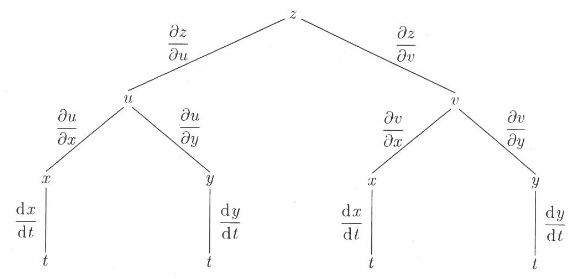
\includegraphics[width=0.6\linewidth]{./lectures/DeepinScreenshot_select-area_20191030114146.png}
\end{figure}

So we have 
\begin{align*}
\frac{dz}{dt} &= 
  \frac{\partial^{}{z}}{\partial{u}^{}}\Big(
    \frac{\partial^{}{u}}{\partial{x}^{}} \frac{dx}{dt}
  + \frac{\partial^{}{u}}{\partial{y}^{}} \frac{dy}{dt}\Big
  ) + \frac{\partial^{}{z}}{\partial{v}^{}}\Big(
    \frac{\partial^{}{v}}{\partial{x}^{}} \frac{dx}{dt}
  + \frac{\partial^{}{v}}{\partial{y}^{}} \frac{dy}{dt}\Big )\\
  &= \Big ( \frac{\partial^{}{z}}{\partial{u}^{}}
    \frac{\partial^{}{u}}{\partial{x}^{}}
    + \frac{\partial^{}{z}}{\partial{v}^{}}
    \frac{\partial^{}{v}}{\partial{x}^{}}\Big ) \frac{dx}{dt} + \Big
    ( \frac{\partial^{}{z}}{\partial{u}^{}}
    \frac{\partial^{}{u}}{\partial{y}^{}}
    + \frac{\partial^{}{z}}{\partial{v}^{}}
  \frac{\partial^{}{v}}{\partial{y}^{}}\Big) \frac{dy}{dt}
\end{align*}

% First 10 mins of the lecture was missed. Update it by watching the lecture
% recording.
%
% TANGENT PLANES

\section{Tangent Planes}
\subsection{Equations for a tangent plane}
Generally for \( z = f(x,y) \) at \( (a,b, f(a,b)) \), we define the
\textbf{tangent plane} to be
\[ 
  z = f(a,b) + f_x(a,b)(x-a) + f_y(a,b)(y-b)
\]
Or
\[ 
  (x,y,z) = (a,b, f(a,b)) + \lambda(1,0, f_x(a,b)) + \mu(0,1, f_y(a,b)),
  \enspace \lambda, \mu \in \mathbb{R} 
\]
Note that \( \lambda = x - a \) and \( \mu = y - b  \) in the latter
expression, you can substitute to check.

\subsection{Directional Derivative}
Define 
$$ f_u (x,y) = \lim_{h \to 0}  \frac{f(x+hu, y+hu_2) - f(x,y)}{h} $$
Where $ ||\underscore{u}||=  1 $. Set $ x = a + hu_1 $, $ y = b + hu_2 $ such that
$ \displaystyle \lim_{h \to 0} (x,y) = (a,b) $ and set $ z(h) = f(x(h), y(h)) $
\par
From the chain rule
$$ \frac{dz}{dh} = \frac{\partial f}{\partial x} \frac{dx}{dh} + \frac{\partial
f}{\partial y} \frac{dy}{dh} $$
$$ = \frac{\partial f}{\partial x} u_1 + \frac{\partial f}{\partial y} u_2 $$
$$ = \Big ( \frac{\partial f}{\partial x}, \frac{\partial f}{\partial y} \Big
  ) \cdot u $$
  \begin{center}
  \fbox{\begin{minipage}{7in}
\begin{example}
    Compute the directional derivative of $ f(x,y) = 4-x^2 - 4y^2 $at (3,-1) in
    the (1,1) direction.
  \begin{align*}
    f(x,y) &= f-x^2 - 4y^2\\
   f_x(x,y) &= -2x \\
   f_y(x,y) &= -8y \\
   f_{(1,1)} (3,-1) &= (f_x(3,-1) , f_y(3,-1)) \cdot \frac{(1,1)}{||(1,1)||} \\
   &= \frac{1}{\sqrt{2}} (-6,8) \cdot (1,1) =  \sqrt{2} 
 \end{align*}
  \end{example}
  \end{minipage}}
  \end{center}
   \subsection{Gradient vector $\nabla f $}
 The gradient vector of $ f $ is a vector with partial derivative compnents 
 $$ \nabla f = (f_x, f_y) = f_x i + f_y j $$
\begin{center}
\fbox{\begin{minipage}{7in}
\begin{example}
 Find the gradient of $ f(x,y) = x^2 - 3(y-1)^2 + 3 $:
\begin{align*}
  \nabla f &= f_x i + f_y j \\
	   &= 2x i - 6(y-1) j
\end{align*}
\end{example}
\end{minipage}}
\end{center}
The gradient $ \nabla f(a,b) $ is perpendicual to the countour line throguh
$ (a,b) $ and in points increasing $ f $. The direction/magnitude of steepest
slope at $ (a,b) $ are given by $ \nabla f(a,b) $ and $ ||\nabla f(a,b)|| $. We can understand these two facts by
 % Basically spans lectures 24,25,26

    % Lecture 27 recorded on the 23/09/19 9:00AM

\section{Differentials}
\subsection{Estimating error}
If the error in $ x $ is most $ E_1 $ and in $ y $ is at most $ E_2 $ then
a reasonanle estimate of the worst case error in the linear approximation of
$ f $ at $ (a,b) $ is 
$$ |E| \approx  |f_x(a,b)E)_1| + |f_y(a,b)E_2| $$

\begin{center}
\fbox{\begin{minipage}{7in}
\begin{example}
Suppose when making up a barrel ofbase radius 1m and height 2m, you allow an
error of $5\%$ in radius and height. Estimate the worst case error in volume

\begin{align*}
  V(r,h) &= \pi r^2 h \;, V(1,2) = 2\pi \\
  V_r(r,h) &= \2\pi rh ,\; V_r(1,2) = 4\pi \\
  V_h(r,h) &= \pi r^2 ,\; V_h(1,2) = \pi
\end{align*}
$$ E_r = \frac{5}{100}r = \frac{5}{100}, \; |E_h| = \frac{5}{100}\cdot 2 = \frac{10}{100} $$
\end{example}
\begin{align*}
  |E| &= |V_r(1,2) E_r| + |V_h(1,2) E_h|\\
      &= 4\pi \cdot \frac{5}{100} + \pi \cdot \frac{10}{100} = \frac{30\pi}{100}
\end{align*}
Now, since $ V(1,2) = 2\pi $ the percentage error is $ \frac{|E|}{V(1,2)}
= \frac{30\pi}{100} \cdot \frac{1}{2\pi} = \frac{15}{100} \equiv 15\% $.
EXACT WORSE CASE SCENARIOS. $ r = 1.05 $, $ h = 2.1 $, $$ \frac{V(1.05,
21)}{V(1,2)} = 1.1576 $$,
$ r = 0.95 $, $ h = 1.9 $, $$ \frac{V(0.95, 1.9)}{V(1,2)} = 0.8579... $$
\end{minipage}}
\end{center}

\subsection{Quadratic Approximation}
Let $ Q(x) = f(a) + f'(a)(x-a) + \frac{f''(a)}{2}(x-a)^2$. Then
\begin{align}
  Q(a) &= f(a)\\
  Q'(x) &= f'(a) + f''(a)(x-a)\\
  Q'(a) &= f'(a)\\
  Q''(x) &= f''(a)\\
  Q''(a) &= f''(a)\\
\end{align}
Eqs (2.1), (2.3) and (2.6) show that $ f(x) $ and $ Q(x) $ are equal at
$ x = a $ as are their first and second derivatives.
\begin{center}
\fbox{\begin{minipage}{7in}
\begin{example}
  Compute $ e^{0.1} $ using a linear and quadratic approximation
\end{example}
For $ f(x) = e^x $, we have the quadratic approximation about $ a = 0 $,
\begin{align*}
  Q(x) &= f(0) + f'(0)x + \frac{1}{2} f''(0)x^2\\
       &= 1 + x + \frac{1}{2} x^2
\end{align*}
Then $ e^{0.1} = f(0.1) \approx Q(0.1) = 1.105 $
\end{minipage}}
\end{center}

\begin{center}
\fbox{\begin{minipage}{7in}
\begin{example}
  In the same graph, sketch $ f(x) = \cos x$ as well as its linear and quadratic
  approximations around 0. (Obviously can't do sketch real time in \LaTeX but
  take photo of graph or watch lecture recording at 9:21am (21 mins))
  Given $ f(x) = \cos x $, $ f'(x) = -\sin x $, $ f''(x) = -\cos x $, $ f(0) = 1 $, $ f'(0) = 0 $, $ f''(0) = -1 $.

  $$ \text{Linear approximation, } L(x) = f(0) + f'(0)x = 1 $$
  $$ \text{Quadratic approximation, } Q(x) = f(0) + f'(0) + \frac{1}{2} f''(0) x^2 = 1 - \frac{1}{2} x^2$$
\end{example}
\end{minipage}}
\end{center}
\subsection{Quadratic approximations}
%The quadratic or second-order approximation to $ f(x,y) $ around $ (a,b) $ is
%a function of the form
$$ Q(x,y) = c+ mx + ny + Ax^2 +Bxy +Cy^2 $$
such that $ Q(a,b) = f(a,b) $ and such that all first order and second order
partial derivatives of $ f $ and $ Q $ agree at $ (a,b) $. To verify
\begin{align*}
  Q(x,y) &= f(a,b) + f_x(a,b)(x-a) + f_y(a,b)(y-b) \\
	 &+ \frac{1}{2}f_{xx}(a,b) (x-a)^2 + f_{xy} (a,b)(x-a)(y-b)
	 + \frac{1}{2}f_{yy}(a,b)(y-b)^2
\end{align*}
\begin{center}
\fbox{\begin{minipage}{7in}
\begin{example}
  Check that $ Q_{xx} (a,b) = f_{xx}(a,b) $ and $ Q_{xy}(a,b) = f_{xy}(a,b) $
  \begin{align*}
    Q_x(x,y) &= f_x(a,b) + f_{xx}(a,b)(x-a) + f_{xy}(a,b)(y-b)\\
    Q_{xx}(x,y) &= f_{xx}(a,b),  \; Q_{xx}(a,b) = f_{xx}(a,b) \\
    Q_{xy}(x,y) &= f_{xy}(a,b) ,\; Q_{xy}(a,b) = f_{xy}(a,b)
  \end{align*}
\end{example}
\end{minipage}}
\end{center}
A more specific example. Bruh moment.
\begin{center}
\fbox{\begin{minipage}{7in}
\begin{example}
  Find the quadratic approximation around $ (0,0) $ of 
  $$ f(x,y) = 1 - x^2 - y^2 + xy  + x^3 + x^2y^2 $$
\begin{align*}
  f(x,y) &= 1 - x^2 - y^2 + xy  + x^3 + x^2y^2, \; f(0,0) = 1 \\
  f_x(x,y) &= -2x + y + 3x^2 + 2xy^2, \; f_x{0,0} = 0\\
    f_y(x,y) &= 2y + x + 2x^2y, \; f_y(0,0) = 0\\
    f_{xx} (x,y) &= -2 + 6x + 2y^2, \; f_{xx}(0,0) = -2 \\
    f_{yy}(x,y) &= 2 + 2x^2, \; f_{yy}(0,0) =2\\
    f_{xy}(x,y) &= 1+ 4xy, \; f_{xy}(0,0) = 1
\end{align*}
The quadratic approximation is
\begin{align*}
  Q(x,y) &= f(0,0) + f_x(0,0)x + f_y(0,0)y + \frac{1}{2} f_{xx}(0,0) x^2\\
  &+ f_{xy}(0,0)xy + \frac{1}{2} f_{yy}(0,0) y^2 \\
  &= 1 - x^2 + xy = y^2 = f(x,y) - x^3 - x^2y^2
\end{align*}
\end{example}
\end{minipage}}
\end{center}


    % Losing track of the Lecture number...
    \section{Constrained optimisation and Lagrange
 multipliers}
\subsection{Lagrange multipliers}
One often needs to maximise or minimise a function subject to certain
constraints.
 
\begin{center}
\fbox{\begin{minipage}{7in}
\begin{example}
Find the minimum value of \( x^2 + y^2 \) subject to the constraint \( x+y
 = 1 \).
\\\\
We want to minimise the function \( f \)subject to the constraint \( x+y = 1 \)
\\\\
We can explicitly solve the \textbf{constraint-equation:} \( y = 1-x\), so
\[ 
   F(x) := f(x,1-x) = x^2 + (1-x)^2 = 2x^2 - 2x+1
\]
Which is a function of \( x \) alone. The critical points of \( F \) occur when
\( F'(x) = -2+4x = 0 \), implying \( x = \frac{1}{2} \). Since \( F''(x)
= 4 > 0 \), it follows that \( F \) has a minimum at \( x = \frac{1}{2}
\). Therefore \( f \) subject to the constraint \( x+y = 1 \) achieves its
minimum value at \( x = y = \frac{1}{2} \) with the actual value also \(
\frac{1}{2} \).
\\\\
You can solve this problem much better without requiring the explicit solution
of the constraint-equation.
\\\\
Define a second function \( g \) such that the constraint-equation corresponds
to \( g(x,y) = 0 \). % Apply more clarity later.
 
In our example, \( g(x,y) = x + y - 1 \). Graphing the contour polot \( f(x,y)
= x^2 + y^2\) and add a graph of the single contour \( g(x,y) = 0 \).
\end{example}
\end{minipage}}
\end{center}


\begin{figure}[h]
  \centering
  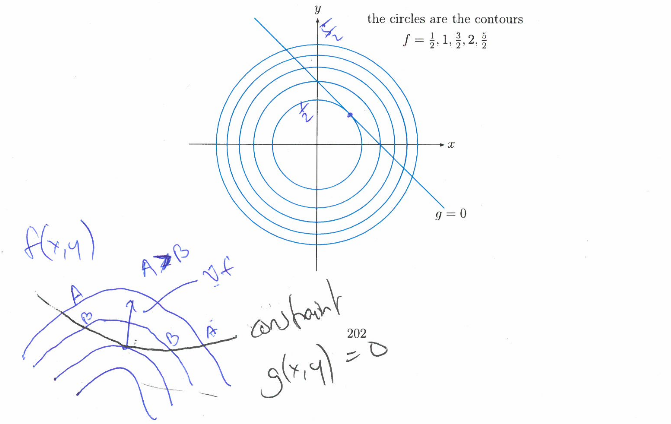
\includegraphics[width=0.6\linewidth]{./lectures/DeepinScreenshot_select-area_20191013194637}
  \caption{}%
  \label{}
\end{figure}

The minimum occurs where the contour \( g(x,y) = 0 \) touches one of the
contours of \( f \), which means that \( \nabla f \) and \( \nabla g \) are
parralel. Hence

\[ 
  \nabla f = \lambda \nabla g
\]
for some \( \lambda \), known as the \textbf{Langrange multiplier}.

\begin{center}
\fbox{\begin{minipage}{7in}
\begin{example}
Find the minimum value of \( x^2 + y^2 \) subject to the constraint \( x+y = 1 \)
\\\\
Let \( f(x,y) = x^2 + y^2 \) and \( g(x,y) = x+y-1 \). We want to minimise \(
f(x,y)  \) subject to the constraint \( g(x,y) = 0 \). Next, \( \nabla
f = (2x,2y) \) and \( \nabla g = (1,1) \). Set \( \nabla f = \lambda \nabla
g \), so \( 2x = \lambda \), \( 2y = \lambda \). Including the constraint \(
g(x,y) = 0 \), this gives us 3 equations in 3 unknowns. The solution is \(
x = y = \frac{1}{2} \), \( \lambda = 1 \). To verify that this is a minimum,
set \( x = \frac{1}{2} + \varepsilon \), \( y = \frac{1}{2}- \varepsilon \)
such that \( x + y = 1 \).
\begin{align*}
  f( \frac{1}{2} + \varepsilon, \frac{1}{2} - \varepsilon) &= \Big( \frac{1}{2}
  + \varepsilon\Big)^2 + \Big( \frac{1}{2} - \varepsilon \Big )^2 \\
  &= \frac{1}{2} + 2 \varepsilon^2
\end{align*}
We see that \( f( \frac{1}{2} + \varepsilon, \frac{1}{2} - \varepsilon) \) is
minimised when \( \varepsilon = 0 \), so (\( \frac{1}{2}, \frac{1}{2} \)) gives
the constrained minimum.
\end{example}
\end{minipage}}
\end{center}

\begin{note}
The following two remarks are important and are direct references to the
workbook.
\end{note}

\begin{remark}
When solving a constrained optimisation problem with Langrange multipliers, it
is typically not necessary to find the value of \( \lambda \). So when solving
your equations obtained from \( \nabla f = \lambda \nabla g\) and the
constraint-equation, your aim is really to \textbf{eliminate} \( \lambda \) in
order to solve for variables in your problem. \\\\
If upon using the method of Langrange multipliers you obtain simple, linear
equations to solve then consider yourself lucky. In some cases you will in fact
obtain nonlinear equations that you need to solve. If this happens we suggest
the first thing you to is try taking the \textbf{ratio} of your equations
obtained from \( \nabla f = \lambda \nabla g \). This allows you to immediately
eliminate \( \lambda \) from your equations and proceed from there. The next
example nicely illustrates this point.
\end{remark}





    \section{Line Integrals}
\subsection{Work done by a constant force}
In a single dimension, work is done by a constant force \( F \) moving an
object along a straight line of length \( d \) is represented as
\[ 
  W = Fd
\]

In two or three dimensions, work done by a constant force in a moving particle
alng a straight line from \( P \to Q\) is 
\[ 
  W = F \cdot \overrightarrow{PQ} = mgd\cos \theta  
\]
\subsection{Work done over a curve}
We now consider the more general case of the work done by a force field
\[ 
  F(x,y,z) = F_1(x,y,z)i + F_2(x,y,z)j + F_3(x,y,z)k
\]
which moves an object along a curve C.
\\\\
First give an approximation, dividing \( C \) into \( n \) arcs such that the
\textit{i}'th arc has length \( \delta s_i \). We approximate \( \delta s_i \)
by evaluating \( F \) at a specified point \( P_i \) on the arc. 


    \section{Central forces}
A force \( F(x,y,z) \) is called central if it has the form:
\[ 
  \textbf{F} = F(r)\hat{ \textbf{r}} = \frac{F(r)}{r} \textbf{r}
\]
where \( \textbf{r} = x\hat{i} + y \hat{j} + z \hat{k} \) and \( r = \sqrt{x^2
+ y^2 + z^2} = (x^2 + y^2 + z^2)^{\frac{1}{2}}\)
Central forces act towards or away from the origin. The maginitude is dependant
on the distance from the origin.
\\\\
Consider the gradient of the radial distance,
\begin{align*} 
  \nabla r &= \Bigg ( \frac{\partial{r}}{\partial{x}},
  \frac{\partial{r}}{\partial{y}}, \frac{\partial{r}}{\partial{z}}\Bigg) \\
	   &= (x^2 + y^2 + z^2)^{\frac{1}{2}} (x,y,z)\\
	   &= \frac{1}{r} \; \underline{r} = \underline{ \hat{r}}
\end{align*}
Let \( F(r) = -\displaystyle \frac{dV}{dr} \) for some function \( V \). We
show that the central force \( \textbf{F}(r) = F(r) \hat{r} \) is conserved
with potential function \( V(r) \).
\begin{proof}

\begin{align*}
  - \nabla V  &= \Bigg(- \frac{\partial{V}}{\partial{x}},
  - \frac{\partial{V}}{\partial{y}}, - \frac{\partial{V}}{\partial{z}}\Bigg)\\
  &= \Bigg(- \frac{dV}{dr} \frac{\partial{r}}{\partial{x}}, - \frac{dV}{dr}
    \frac{\partial{r}}{\partial{y}}, - \frac{dV}{dr}
  \frac{\partial{r}}{\partial{z}}\Bigg) \;\; (\text{By the chain rule}) \\
  &= F(r) \Bigg( \frac{\partial{r}}{\partial{x}},
  \frac{\partial{r}}{\partial{y}}, \frac{\partial{r}}{\partial{z}}\Bigg)
  = F(r) \hat{r}\\
  \frac{dE}{dt} &= \frac{1}{2}m \underline{ \dot{v}} \cdot \underline{v}
+ \frac{1}{2} m \underline{v} \cdot \underline{ \dot{v}} + \frac{dV}{dr}
\dot{r} = m \underline{a} \cdot \underline{v} + \frac{dV}{dr} \dot{r} 
\end{align*}
Therefore all \textbf{central forces are conservative} (provided that \(
\textbf{F}(r) \) is integrable). Hence a particle moving in a central force \(
\textbf{F}(r) = -V'(r) \hat{r}\) has energy
\[ 
  E = \frac{1}{2} mv^2 + V(r)
\]
which remains constant.
\end{proof}
\section{Angular Momentum}
A particle with mass \( m \), velocity \( \textbf{v} \) and position \(
\textbf{r} \), then the angular momentum is given by
\[ 
  L = m( \textbf{r} \times \textbf{v} )
\]
A force exerted on the particle, by Newton's Second Law.
\begin{align*}
  \underline{\dot{L}} &= m( \underline{\dot{\textbf{r}}} \times
  \underline{\textbf{v}}) + m( \underline{ \textbf{r}} \times \underline{ \dot{
  \textbf{v}}}) \\
  &= m ( \underline{ \textbf{v}} \times \underline{ \textbf{v}}) + m(
  \underline{ \textbf{r}} \times \underline{ \textbf{a}})\\
  &= \underline{ \textbf{r}} \times \underline{ \textbf{F}}
\end{align*}
We call \( \textbf{r} \times \textbf{F} \) the \textbf{torque} for a central
force \( \textbf{F} = \displaystyle \frac{F(r)}{r} \textbf{r} \). So the time
derivative is 
\begin{align*}
  \underline{ \dot{ \textbf{L}}} = \textbf{ \underline{r}} \times \underline{
  \textbf{F}} &= \frac{F(r)}{r} ( \underline{ \textbf{r}} \times \underline{
\textbf{ r}}\\
  &= 0
\end{align*}
As \( \textbf{L} \) is constant (it's not gonna change anytime soon), we have
\textbf{conservation of angular momentum}. Also as angular momentum is a vector
quantity \( \implies \) that both the magnitude and direction is constant as
well.
\\\\
\textbf{By the definition of the cross product, the direction of the angular
momentum is perpendicular to the position and velocity vectors.}
\\\\
This means that motion is confined to a plane. \textbf{Without any loss of
generality}, we can choose this plane to be the \( x-y \) plane.
\section{Polar Coordinates}
Its natural to represent central force problems in polar coordinates in \(
\mathbb{R}^2 \). These are an example of \textbf{curvlinear coordinates}. The
basic vectors used in curvlinear coordinates are \textbf{not} fixed in space.
They change according to a position of a particle. 
\begin{example}
One basis vector is given by
\[
  \hat{ \textbf{r}} = \cos(\theta) \hat{i} + \sin(\theta) \hat{j}
\]
We can check that a perpendicular unit vector is given by
\[ 
  \hat{\theta} = - \sin(\theta) \hat{i} + \cos(\theta) \hat{j}
\]
The vectors \( \underline{ \textbf{r}} \) provide an orthogonal basis for \(
\mathbb{R} ^2 \). We need to to check if the following two properties hold
\begin{enumerate}
  \item \[\frac{d \hat{r}}{d\theta} = \hat{\theta}\]
  \item \[\frac{d \hat{\theta}}{d\theta} = -\hat{r}\]
\end{enumerate}

We can obtain the following expressions for the velocity and acceleration

\begin{align*}
  \underline{r} &= r \underline{ \hat{r}}\\
  \underline{v} = \underline{ \dot{r}} &= \dot{r} \underline{ \hat{r}}
  + r \frac{d \underline{ \hat{r}}}{dt}\\
  &= \dot{r} \underline{ \hat{r}} + r \frac{d \hat{r}}{d\theta}
  \frac{d\theta}{dt}\\
  &= \dot{r} \underline{ \hat{r}} + r \dot{\theta} \underline{ \hat{ \theta}}
\end{align*}
For the acceleration
\begin{align*}
  \underline{a} &= \frac{d \underline{v}}{dt}\\
  &= \ddot{r} \underline{ \hat{r}} + \dot{r} \frac{d \underline{ \hat{r}}}{dt}
  + \dot{r} \dot{\theta} \hat{\theta} + r \ddot{\theta} \hat{\theta}
  + r \dot{\theta} \frac{d \hat{\theta}}{dt}\\
  &= \ddot{r} \underline{ \hat{r}} + \dot{r} \frac{d \underline{
  \hat{r}}}{d\theta} \dot{\theta} + \dot{r} \dot{\theta} \hat{\theta}
  + r \ddot{\theta} \underline{ \hat{\theta}} + r \dot{\theta} \frac{d
  \underline{ \hat{\theta}}}{d\theta} \dot{\theta}\\
  &= ( \ddot{r} - r \dot{\theta}^2) \underline{ \hat{r}} + (2 \dot{r}
  \dot{\theta} + r \ddot{\theta}) \underline{\hat{\theta}}  
\end{align*}
We are dealing with a central force \( \textbf{F} = -V'(r) \hat{r} \) such that
the equation of motion is
\[ 
  -V'(r) \hat{r} = m( \ddot{r} - r \dot{ \theta}^2) \hat{r} + m(2 \dot{r}
  \dot{\theta} + r \ddot{\theta}) \hat{\theta}
\]
Equating the radial and angular components. For the radial part.
\[ 
  \ddot{r} - r \dot{\theta}^2 = - \frac{V'(r)}{m}
\]
And for the angular equation
\[ 
  2 \dot{r} \dot{\theta} + r \ddot{\theta} = 0;
\]
Rewriting the angular equation we have
\[ 
  \frac{d}{dt}(r^2 \dot{\theta}) = 0
\]
This is saying that the magnitude of angular momentum is constant over time.
I.e 
\[ 
  L = mr^2 \dot{theta}
\]
Where \( L \) is constant. We can describe the motion of the particle by the
radial equation
\[ 
  \ddot{r} = \frac{L^2}{m^2r^3} - \frac{V'(r)}{m}
\]
\end{example}
\section{Circular Motion}
Attractive central forces are capable of producing circular motion moving at
constant speed. Given for circular motion, \( r \) is constant \( \implies
\dot{r} = \ddot{r} = 0 \). We have
\begin{align*}
  v^2 &= ( \dot{r} \underline{\hat{r}} + r \dot{\theta}
  \underline{\hat{\theta}})\cdot( \dot{r} \underline{\hat{r}} + r \dot{\theta}
  \underline{\hat{\theta}})\\
      &= \dot{r}^2 + r^2 \dot{\theta}^2\\
      &= r^2 \dot{\theta}^2 = \frac{L^2}{mr^2}
\end{align*}
The value of \( L \) is given by the explicit knowledge of the potential. Since
\( \ddot{r} = 0 \),
\begin{align*} 
  0 &= \frac{L^2}{m^2r^3} - \frac{V'(r)}{m}\\
  L^2 &= mr^3V'(r)  
\end{align*}
Which gives \( v^2 = \displaystyle \frac{rV'(r)}{m}\)
\begin{example}[A rotation spring without damping]
Consider a spring of length \( l  \) and spring constant \( k \), with a mass
attached at one end and fixed at the origin. The system sits on a frictionless
table and is able to rotate about the origin in the horizontal plane. This is
a central force problem where
\[ 
  F(r) = -k(r-l) \;\;\;\; V(r) = \frac{k}{2}(r-l)^2
\]

\begin{figure}[h!]
  \centering
  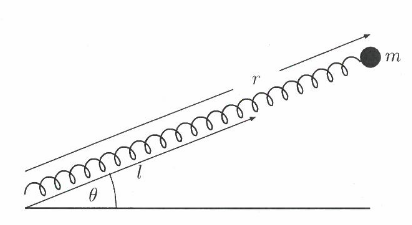
\includegraphics[width=0.4\linewidth]{./lectures/fig.png}
\end{figure}
For \( r > l \), circular motion occurs with \( \dot{r} = 0 \) and \(
v = \displaystyle \sqrt{\frac{kr(r-l)}{m}} \). Otherwise the motion is
determined by the solution to the ODE.
\[ 
  \dot{r} = \frac{L^2}{m^2r^3} - \frac{k(r-l)}{m}
\]
\end{example}
\section{The envelope of a family of functions}

Consider a function of two variables \( f(x,t) \), we can intepret this
funcition as a family of one variable functions by setting
\[ 
  y^{(t)}(x) = f(x,t)
\]
\\\\
...
\\\\
How does the concept of the envelope arises in economic modelling? Suppose that
a bakery's weekly bread roll production is described by \( f(x) \) (given the
conditions for \( x \leq 0 \) that \( f(0) = 0, f(x) \leq 0 \), \( f'(x) > 0 \)
and the cost of one kg of flour be \( c \), the selling price for one kilogram
of bread rolls is \( p \). We will consider \( p \) to be a variable, while \(
c\) is a constant. The profit \( P(p,x) \) is given by
\[ 
  P(p,x) = pf(x) - cx
\]
It is straightfoward to verify that the cross section of \( P(p,x) \) in \(
p  \)havve a local maximum when
\[ 
  f'(x) = cp^{-1}
\]
Specifically
\begin{align}
  P_x(p,x) &= pf'(x) - c\\
  P_{xx}(p,x) &= pf''(x)
\end{align}
When \( f'(x) = cp^{-1} \), Eq. (3.1) shows that a cross-section of \( P \) in
\( p \) has a critical point. Also since, \( f''(x) < 0 \), Eq. (3.2) shows
that the critical point is al local maximum.
\\\\
Let \( x = g(p) \) be the solution for (3). We define the maximised profit
function \( f^{max} \) by 
\[ 
  f^{max}(p) = pf(g(p)) - cg(p)
\]
This is the envelope of \( P(p,x) \) with the property
\[ 
  \frac{dp^{max}}{dp} = f(g(p))
\]

\begin{enumerate}
  \item \( f(x) = 4x^{1/2} \)
  \item \( f(x) = \frac{x}{x+1} \)
\end{enumerate}

both of which satisfy the required conditions for \( x \leq 0 \mid f(0) = 0,
f(x) \leq 0, \; f'(x) > 0 \) \( f''(x) < 0 \).

\begin{align*}
  f(x) &= 4x^{ \frac{1}{2} }\\
  f'(x) &= 2x^{-\frac{1}{2}} = cp^{-1} \implies x = g(p) = \frac{4p^2}{c^2}\\
  f(g(p)) &= 4 \sqrt{ \frac{4p^2}{c^2}} = \frac{8p}{c}\\
  \intertext{Then}
  p^{max} (p) &= \frac{8p}{c} \times p - c \Big( \frac{4p^2}{c^2}\Big )
  = \frac{4p^2}{c}
\end{align*}







    
    \end{document}
